\documentclass[letterpaper,twocolumn,10pt]{article}

\usepackage{usenix,authblk}
\renewcommand\Affilfont{\itshape\small}
\usepackage{graphicx}
\usepackage{url}
\usepackage[toc,page]{appendix}

\makeatletter
\newcommand\appendix@section[1]{%
  \refstepcounter{section}%
  \orig@section*{Appendix \@Alph\c@section: #1}%
  \addcontentsline{toc}{section}{Appendix \@Alph\c@section: #1}%
}
\let\orig@section\section
\g@addto@macro\appendix{\let\section\appendix@section}
\makeatother

% Hi Everyone, we can start with this template Cynthia gave us and go from here
% The comment feature is great for annotating text, use it!
% pdflatex should compile this just fine for now

% This file will be the main file, I just splitted the sections in different latex files, so we can modify any section in an easy and simple way. I joined all the sections in the paper using the \input{filename} command.
\begin{document}

\title{Automated Election Auditing From DRE Logs}
\author[1]{D. Wagner}
\author[1]{C. Sturton}
\author[2]{A. Edmundson}
\author[3]{K. D. Ortiz}
\author[4]{A. M. Quevedo}
\author[5]{S. Rodr\'{i}guez}
\author[6]{P. Baxter}

\affil[1]{University of California-Berkeley}
\affil[2]{Cornell University}
\affil[3]{University of Puerto Rico-Arecibo}
\affil[4]{Miami Dade College}
\affil[5]{University of Puerto Rico-Mayag\"uez}
\affil[6]{Clemson University}

% Add additional authors:
% \and Author n
\maketitle

%Abstract

%Changes here (in the main paper I'll just invoke this file)
\subsection*{Abstract}
Voting audit logs produced by electronic voting systems contain information that is useful for uncovering procedural errors and election anomalies, but are currently unwieldy and difficult for election officials to use in post-election audits. In this work, we developed new methods to analyze these audit logs that includes the detection of both procedural errors and system deficiencies. We created a public web application that applies these methods to generate useful feedback on any detected issues. Election officials can use our tool to identify memory cartridges containing precinct totals that were not uploaded on election night, machines that may have experienced hardware problems during the election, and polling locations that closed late or had voters waiting in line for extended periods. We tested our analyses on data from the South Carolina 2010 elections and were able to uncover solely through the analysis of audit logs that there were 1127 votes not counted in the certified totals in Richland County, South Carolina.

%Introduction section
\section{Introduction}
Your intro goes here.

\subsection{Sub-section title}
Maybe your introduction has subsections.

%Background section
\section{Background}
\label{sec:background}
\subsection{Introduction to the iVotronic DRE}
A brief description of the iVotronic's functionality and its main
system components follows. 

\begin{itemize} 
\item \textbf{Voting terminal.} The voting terminal is a stand-alone
  touchscreen voting unit.  The terminal is equipped with an internal
  battery, which keeps the unit operational in the event of a power
  failure, and a removable compact flash card, which is used to store
  audit data and ballot images (cast vote records). Typically, each
  polling location is assigned several iVotronic machines. Also, to
  comply with the federal American with Disabilities Act, at least one
  audio terminal is placed in each precinct to assist disabled
  voters. 

\item \textbf{Personalized Electronic Ballot (PEB).} The PEB is a
  proprietary cartridge designed by ES\&S to operate the iVotronic
  terminal.  When the PEB is placed in the machine, the terminal and
  the PEB can communicate through an infrared port.  Typically,
  counties deploy two types of PEBs to the precinct: a) a master PEB
  and b) an activator PEB. Both types of PEBs have the same
  functionality, however, poll workers are trained to keep them
  separate and use them for different purposes. 
    \begin{itemize}
    \item \textbf{Master PEB.}  Poll workers use the master PEB to
      open polls on election day. When the PEB is placed in the
      terminal, the touchscreen displays the precinct's name
      programmed in the PEB so that poll workers can verify the
      polling location information and date/time registered in the
      terminal's internal clock. If the information displayed is
      correct, the poll workers open the terminal for voting. The same
      master PEB should be used to open all terminals in the polling
      location. In the same fashion, the master PEB should be used to
      close all terminals in the polling location at the end of the
      voting day. When a terminal is closed, it uploads its vote
      totals onto the PEB inserted into it. When the master PEB is
      used to close all terminals, this PEB accumulates the precinct
      totals so that they can later be uploaded and included in the
      official tally. 
    \item \textbf{Activator PEBs.}  Activator PEBs are used by  poll
      workers to activate ballots for voters. Election officials
      provide each precinct with multiple activator PEBs.  
    \end{itemize}
\end{itemize}
Internally, all PEBs at the precinct are identical. The only
difference between them is the color of the rubber band on their
exterior. Thus, a master PEB can be used to activate a voter's ballot
and an activator PEB can be used to open and close terminals. Though
as a matter of procedure and training, they should not be used this
way. If an activator PEB is used to close terminals, the precinct vote
totals may be only partially uploaded to the aggregated totals on
election night. Poll workers are trained so that they put the master
PEB, CF cards and precinct's totals tapes in a designated bag that is
transported to Election Central after polls close.  Activator PEBs
used to close terminals may be left behind and their vote data not
added to the certified count.
\begin{itemize}
\item \textbf{Removable Compact Flash (CF) card.} The CF cards are
  programmed at Election Central and installed in the back of the
  voting terminal prior to deployment at the polling location. The CF
  cards contain graphic (bitmap) files read by the voting terminal
  during the voting process. The CF cards are also used as an external
  memory device: audit log entries and ballot images are written to
  the CF card when the terminal is closed for voting. Once the polls
  close, the CF cards are removed from the back of the terminal and
  delivered to election headquarters on election night.  

\item \textbf{External printer module.} This module is connected to a
  serial port on the back of the voting terminal. The thermal printer
  produces the precinct zero tape and results tape. Poll workers are
  instructed to print the zero tape once all iVotronics of the polling
  location are opened for voting. In the same fashion, they are
  trained to print the results tape when all voting terminals are
  closed on election night. 
\end{itemize}

\subsection{iVotronic Audit}
The ES\&S voting solution produces many log files including the
Election Reporting Manager (ERM) \textquotedblleft System
Log\textquotedblright \hspace{1 mm} file, the ERM \textquotedblleft
Result Correction Log,\textquotedblright \hspace{1 mm} the ERM
\textquotedblleft Real Time Log,\textquotedblright \hspace{1 mm} the
iVotronic \textquotedblleft Ballot Image\textquotedblright \hspace{1
  mm} log and the iVotronic \textquotedblleft Event
Log.\textquotedblright \hspace{2 mm} We focus on three: the event log
(EL152.lst), ballot image file (EL155.lst), and the system log
(EL68a.lst).  The header of these log files identify the county's
name, the type and date of the election, the date the report was
generated, and the election ID. The election ID is a parameter
generated by the ES\&S election programming software to uniquely
identify each election.  
 
The event log (EL152.lst) contains audit log entries from each
iVotronic terminal used in the election.  The log  records, in
chronological order, all events that occurred on that machine during the
election. It typically begins at election headquarters, before the
election, with a \textquotedblleft clear and
test\textquotedblright \hspace{1 mm} of the terminal to delete
previous election data from the terminal's memory. It also records all
election day events, including polls open and polls closing and the
number of ballots cast.  Each event log entry includes the iVotronic's
terminal serial number, the PEB's serial number, the date and time,
the event that occurred and a description of the event. An excerpt of
an event log is given in  Appendix~\ref{app:el}. 
 
The ballot image file (EL155.lst) contains all ballot images saved by
the iVotronic terminals during the voting process. An ES\&S ballot image
is a list of all choices made for each vote cast; it is not a scanned
or photographic image. The ballot images are segregated by precinct and
terminal where the votes were cast. The ballots are saved in a random
order to protect the privacy of the voter.  An excerpt of a ballot image
file is given in Appendix~\ref{app:bi}
 
The system log listing file (EL68a.lst) chronologically tracks activity
in the election reporting database at the election headquarters. Its
entries reflect the commands executed by the operators during
pre-election testing, election night reporting, post-election testing
and canvassing. It also contains the totals accumulated in the various
precincts during election night reporting, as well as any warnings or
errors reported by the software during the tabulation process.
The system log also tracks the uploading of PEBs and CF cards to the
election reporting database. Manual adjustment of precinct totals are
also recorded in the system log file. An excerpt of a system log file is
given in Appendix~\ref{app:sl}. 

%Analyses section
%Invoke the sub-sections through the input{filename} command.
\section{Analyses}
In this section we present a description of our analyses and important findings.  The iVotronic log files used for testing these analyses were downloaded from the website titled ``South Carolina Voting Information'' % Footnote the url \url{scvotinginfo.com}.
\subsection{Votes Possibly Not Counted}
\subsubsection{PEBs Not Uploaded}
Currently, the election officials performing the vote tabulation on election night do not have a way to effectively compare the list of PEBs that have been successfully uploaded to the tabulation software with the pool of PEBs containing vote data throughout the county. This can lead to inaccuracies in election results if any PEBs containing vote data are accidentally left out of the tally process. Our tool provides an analysis that generates a list of PEBs used to collect votes on election day. It warns election officials of any PEB, master or non-master, that was used to close a terminal, whose data wast not uploaded to the election reporting system.   

The precinct procedures for poll workers dictate that a single PEB should be used to open and close all machines at a polling location. Failure to strictly follow this protocol led to problems in Miami-Dade County during the 2002 Primary election~\cite{Mazella2002}. In that case, poll workers used two or more PEBs to open and close terminals at their precinct.  However, election workers at county headquarters only uploaded one of these PEBs, expecting all machines to be closed with the same PEB. This caused a significant delay in the reporting of election results. A recent study found similar problems in several South Carolina counties~\cite{Buell2011}.

This analysis is specific to the iVotronic system. It requires the event log, the ballot image file, and the system log. The event log records the serial number of the PEB used to close the terminal.  It also records, in chronological oder, vote events processed in the voting machine. The system log file tracks a running log of the serial number of PEBs uploaded to the ERM tabulation system. The ballot image file provides a list of terminals used in each precinct.

Our method keeps track of the serial number of the PEB used to close each voting machine. It also records the polling location each voting machine was assigned to as well as the total votes cast in each machine. Then,  it verifies that each PEB that was used to close voting machines is uploaded to the ERM vote tally. It reports any PEB containing vote data that has not been added to the cumulative count.  For each such PEB, our analysis reports the serial numbers of the terminals collected by the PEB, the number of votes processed in those terminals and the precinct's name and number. With this information, election officials can gather the missing PEBs and collect votes from terminals not included in the cumulative totals.

\subsubsection{Machines Not Closed}
There are two main pieces of the election system that need to be analyzed to determine if votes were left out of the count.  We have discussed the first essential piece: the PEB.  The second piece of the election system that must be taken into account is the voting machine itself.   We have devised a way to determine which machines have not been closed for voting.  If a machine is not closed, then a PEB has not collected this terminal's data; our algorithm will help detect this situation where some votes were not counted.  

This analysis uses the event log and the ballot image file to provide feedback; the event log should have the ability to record events marking the opening and closing of each voting machine.  The ballot image file allows us to identify which machines were at each polling location.  We created a method that checks if a machine was closed, given it was also opened for voting.  Our analysis searches through the event log for machines that were opened; these machines are stored in a data structure.  Next, we check that every machine in the data structure also recorded an event representing its closure.  If there are any machines that have been opened and not closed, they are displayed to the election official.   

\subsection{Incomplete Audit Data}
Due to the manner in which both the event log and the ballot images file are created, they may not include all audit data.  When a machine occurs in the event log with recorded votes cast on it during election day, but does not appear in the ballot images file, this indicates that some ballots are missing from the ballot images file.  The reverse situation reveals the opposite error- the event log is not complete.  We developed a technique that identifies incomplete files.  

This analysis requires an event log and a ballot images file, where both files record machine serial numbers for any events and ballots cast.  Our analysis crosschecks these files for inconsistencies that may reveal unforeseen problems.  In our algorithm, we create two data structures; the first contains every machine used for voting and how many votes were cast on it according to the event log, the second contains every machine with ballots cast on it and how many ballots were cast on it according to the ballot images file.  Then, we compare these two structures.  Ideally, they would have the same contents and we could conclude that the files are consistent.  However, there may be cases where one file has a machine with more votes on it than the other file�s corresponding machine.  In this case, we would report file inconsistencies and provide the user with the machine serial number and the conflicting vote counts.   

\subsection{Polling Location Related Analyses}
\subsubsection{Polling Locations that Closed Late}
In the United Stated, poll hours are regulated by the state
officials. Poll closing hours vary from 6pm to 9pm depending on the
state~\cite{Info2007}. Some state statutes allow the voters waiting in
line at poll closing time to cast their ballots at the precinct;
therefore, polling locations may stay open late in order to
accommodate those voters waiting in line at the official poll closing
time. If election officials knew which polling places were likely to
experience long lines they could deploy more equipment or personnel to
those locations. This analysis can assist them by providing
information about long lines that occurred in the current election. Election
officials can use this information to make predictions about where
long lines might occur in future elections of the same type. 

This analysis gathers the time each machine was closed from the event log and the precinct the machine was assigned to from the ballot image file; to perform the analysis, this data is required.  Our algorithm saves this information in a data structure and generates a countywide chart detailing the number of polling locations that stayed open after poll closing time and for how long. To handle inaccurate machine date/time settings, our tool uses a time verification algorithm described in Section 3.6 to exclude from our database any voting machines whose time stamp is probably incorrect. 

\subsubsection{Long Lines}
Election officials assign voting machines and supplies to each polling
location based on the number of voters registered in the precinct.
However, voter turnout can vary and as a result, some polling
locations may end up overstocked with equipment, supplies or poll
workers while others may lack resources on election day. As a result,
voters may have to wait in line before casting their vote. This is
common during mid-term and general elections~\cite{Kreitman2010,
  Slade2008, U2010}, as well as any elections with high-voter turnout.
In those circumstances, election officials might like information
about which locations experienced long lines and at what time of the
day. However, monitoring all the polling places in a large county can
be a daunting task. Therefore, we provide an analysis that can analyze
DRE audit data to identify peak times at the precincts. Such
information can assist election officials with the planning of
resource allocation for future elections.

This analysis reports busy locations by detecting heavily used voting terminals. It requires an event log that captures every vote cast event along with an accurate time stamp and precinct location information. In our analysis we find this information in the event log and the ballot image file. When there are consecutive ballots cast in all machines in a polling location with no time delay in between, we are able to infer that there is a steady flow of voters and possibly a line of voters waiting to use the voting machines. 

However, the analysis is not quite so straightforward. The event logs
we used captured the \textquotedblleft cast vote'' event, but that
only tells us when the voter finished making their selection. In order
to know if there is any idle time between voters, we would also need
an event that notes when a new ballot is loaded into a machine. The
idle time would be the time between one \textquotedblleft cast vote''
event and the next \textquotedblleft ballot loaded''
event. Unfortunately our logs have no such \textquotedblleft ballot
loaded'' event. Instead, we had to infer the idle time. We did this by
focusing on the polling locations which stayed opened after poll
closing time as we could conclude they were busy processing the voters
standing in line at that time and the time between cast vote events
includes no idle time. For those locations, we measure the time it
took voters to cast ballots during the extended poll hours. We also
calculate and keep track of the time per ballot cast during regular
poll hours. Using the Kolmogorov- Smirnov statistical test we can
determine whether the distribution of time between vote cast events
during regular poll hours, in one-hour time windows, matches the
distribution of time between vote cast events during the extended poll
hours. If the distribution of the two samples is consistent, we can
infer the possibility of long lines during the particular one-hour
time period. \footnote{The KS test starts with the null hypothesis
  that the two samples come from the same distribution, which is the
  situation we are interested in identifying. Therefore, the most we
  can say in the case that the null hypothesis cannot be rejected is, we
  cannot reject the possibility that there were long lines between a
  particular time window.} 

\subsection{Hardware Issues}
Election officials may be interested in identifying machines that have hardware problems, such as screen calibration issues, machines with a low battery, terminals that closed early, and machines that recorded unknown, but possibly severe events.  The first of these analyses detects machines with recurring calibration errors and machines that had recorded votes while possibly not calibrated.  By finding the events that correspond to a screen that is not calibrated and to the recalibration of that screen, we can find if votes were cast in between those times.  The second analysis regarding hardware issues looks for machines with an unusually large number of events titled \textquotedblleft Terminal shutdown - IPS Exit\textquotedblright .  We infer that these machines have a low battery because they experience a more-than-normal number of events related to the Internal Power Supply.  Additionally, our tool searches for machines that recorded a warning event about the terminal closing early.  In order for this event to occur, a trained technician must enter a password to access the service menu and make a particular selection to close the machine.  If a machine is closed in this manner during election day, there must be something wrong with it that is preventing votes from being cast correctly.  Lastly, there is a set of events that have questionable meanings, but could potentially represent hardware issues.  

Analyses such as these can help officials identify machines that may require maintenance or to be replaced.  In the case of a machine having ballots cast on it when it is not calibrated, it may not have captured the voter's intent.  Depending on the magnitude of the situation, this could cause a different outcome in the election.  If our analyses detect other hardware problems with a machine, it may not be recording votes accurately; these votes may not even appear in the event log or ballot images.  If the event log and the ballot images do not record ballots being cast, then it is nearly impossible for officials to realize votes are not being counted.  

Due to the available resources and the nature of these analyses, assumptions were made regarding the meaning of events and the severity of the situation.  Currently, there is no user manual or detailed description of the events that appear in the event log; because of this, we are not able to guarantee that the event \textquotedblleft Terminal shutdown - IPS Exit\textquotedblright means the machine has a low battery.  This assumption is also applicable to our calibration analysis and our detection of unknown warning events.  If a description of each event was available, we could be more definitive in our results and possibly implement analyses that report other useful hardware failures.    

The machines used in South Carolina have experienced frequent potential hardware issues.  For example, the combination of machines in Berkeley County experienced votes cast on a machine when the machine was not calibrated, machines with possible low batteries, and at least one machine that closed early.  Our analysis found that there were seven counties where at least one machine was possibly not calibrated when vote(s) were cast on that machine; these errors spanned 12 different polling locations.  We suggest an election official or technician inspect these machines for possible calibration issues.  We had similar findings when searching for terminals that recorded a "Warning - Terminal Closed Early" event.  There were machines with this warning in seven counties and 13 polling locations.  Terminals should not close before 7 P.M. in South Carolina on election day; for this reason, we recommend that these machines be evaluated for potential problems that would have caused early closure.  When our tool reports machines with possible low batteries, election officials should verify that the machine is working properly and does not need maintenance.  Florence County and Greenville county experienced a number of Internal Power Supply - related events; at least one machine in each precinct had 53 and 63 instances of this event, respectively.  This could be a possible indicator that the battery is running low; therefore, the election officials should take action to ensure all machines work properly in future elections.  

\subsection{Procedural Errors}
It may be beneficial to election officials if they could detect at which locations poll workers are following the required procedures.  Procedural errors can cause many problems including lost votes, incorrect vote counts, disgruntled voters, and long lines.  A few of these are: precincts that do not print zero tapes on the morning of election day; using a master PEB to activate ballots; opening and closing machines with different PEBs.  
If election officials are aware of the procedures that are not being followed, they could review their precinct checklist.  This will allow for more efficient audits as well as a better voting experience for voters.  

\subsubsection{Printing Zero Tapes}
According to the South Carolina poll worker training video (citation), poll workers are required to print at least one zero tape per polling location on the morning of the election.  Using the event log, our tool checks each polling location for this event and reports the locations that did not record this event.  

\subsubsection{Ballot Activation with a Master PEB}
Another way our tool finds procedural errors is by crosschecking the master PEBs with the PEBs used to activate ballots.  Poll workers should be using non-master PEBs to activate ballots so that the PEBs do not get switched.  

\subsubsection{Opening and Closing a Machine with Different PEBs}
Along the same lines, we report incidents of opening and closing a machine with different PEBs.  A machine should be opened and closed with the same master PEB; if not, it may be more likely that this PEB does not get uploaded.   

\subsubsection{Anomalous Vote Cancelled Events}
When poll workers cancel ballots, they must select a reason why; this is another way to detect errors.  There are seven options for canceling a ballot: wrong ballot, voter left after the ballot was issued, voter left before the ballot was issued, voter request, printer problem, terminal problem, or an unspecified reason.  If there are any instances of canceling a ballot due to a printer problem, it could be an indicator of a procedural error because ballots are not printed.  In other cases, if there is a large number of a specific reason, such as having the wrong ballot, this could indicate the poll workers are repeatedly issuing the wrong ballot.  




\smsubsection{Systematic Date and Time Errors}\label{an:date} 
\smvertspace
Correct time-stamps in the audit logs
are critical in post election audits as any incorrect time-stamps
could preclude further log analysis. 
We classify time-stamp errors into two categories: errors
resulting from incorrectly set clocks and errors resulting from apparent bugs in
the time-stamp mechanism itself. Our tool will analyze log files to
find and report errors of each category type.

This analyses requires that each event in the audit log
is marked with a time-stamp based on the machine's internal clock. If
the clock can be manually set, we require that any adjustment made to
the clock is recorded as an event in the
audit log. Additionally, opening and closing events recorded in the logs proved
useful to the analysis. It allowed the analysis to report only those
errors that occur on election day and to avoid reporting as error
any inconsistent time-stamps that occur prior to election day and are
likely the result of pre-election testing or configuration of the
machines. We developed some checks to report if any of
the above requirements are not met by the log data.

Often, an analysis of the time-stamps can produce ambiguous
results. For example, if a machine has its clock set an hour back it
is difficult to determine, from the log files alone, whether the machine
was opened early or its clock was incorrectly set. In our analysis, we
favor accurate identification of date errors over complete
identification. We want to avoid flooding the user with false or
ambiguous error reports. For this reason, we developed techniques to
remove as many ambiguities as possible and report only those
instances which we can positively identify as errors.

We perform these analyses by sequentially parsing each event in the
audit log while looking for events marking a manual clock adjustment
or an erroneous shift between two consecutive time stamps. We explain
our technique further in the following subsections.

\smsubsubsection{Incorrectly Set Dates}
This report identifies any machine that opened for election day voting
with an incorrectly set clock.  This means the opening event and
possibly all subsequent vote events were recorded with incorrect
time-stamps. This error can prevent other analyses
from properly detecting how long the polls stayed open, whether they opened on
time, or if they experienced long lines. Additionally, it may be useful for an
election official to identify counties or precincts where these errors were
particularly common so that pre-election testing procedures can be improved.
We used two different detection algorithms to identify these errors.

The first found machines that opened for voting with wildly incorrect
dates and times. In this algorithm we looked for any machine which
opened for election day voting on any date after the official election
day or any date more than one month prior to election day. This one
month threshold allowed us to avoid reporting those machines which
were legitimately opened, possibly for early voting, on a date before
the official election day. \cks{Patrick, is this the right reason for
  the one month window? Correct it if I'm wrong.}

The first algorithm found those machines whose date and time were
off by a large amount, but it will not find machines that have a
time-stamp that is off by only a small amount, perhaps just an
hour. To find those machines we used a different technique. Instead of
looking at the time of opening or closing, we instead looked for
machines whose time-stamp was manually adjusted at some point while
the machine was opened for voting. If we saw an event indicating the
time-stamp was set forward one hour, for example, we could surmise that
up until that point, the machine's clock had been one hour slow and we
could retroactively adjust the time-stamps of the earlier events for
use by our other analyses.

If a machine opens with a clock that is wrong, but by an amount
smaller than our allowed window of error (one month for slow clocks,
24 hours for fast clocks), and whose clock is not adjusted at any
point during election day, our analyses will fail to catch the
error. We decided on this window size after some trial and error with
the South Carolina data set we were working with; this size seemed to
yield the fewest false positives while still returning useful
results. Possibly, other data sets will require a different
window. This analysis could reasonably be parametrized to
allow the user to specify the desired window size if the default does
not provide useful results.

\smsubsubsection{Datetime Errors}
This report identifies anomalies in the time stamps that are not a result
of human error. In the course of our analysis of the South Carolina
data set, we found many dates that changed, seemingly at random and without
a manual date adjustment event. Sometimes these jumps were temporary
and the clock would jump back to its original time, other jumps
appeared to be permanent. These occurrences suggest an issue with the
machine itself rather than a procedural error. The cause of these errors remains
unknown, but it is concerning that these values can change arbitrarily
as they have the potential to invalidate other audit analyses.  Reporting these
anomalies may assist officials in determining which machines require
inspection by the DRE vendor.

Since events are appended in chronological order, any time-stamp that decreases
chronologically without a corresponding event indicating a manual
adjustment took place is an error and is detected by this
analysis. Forward jumps in time are not necessarily the result of an 
inconsistent time record; a machine can be shut down in a hibernation state for
weeks between events. However, given the relatively short duration of elections, jumps
forward in time, that are past a certain threshold, can reasonably be considered
erroneous. The algorithm looked for deltas between time-stamps that jump
forward by more then 33 days. With the South Carolina data set we
analyzed, this threshold seemed to
avoid including machines that were simply in hibernation between the
factory setup and election day voting. Additionally, some machines were found to have their clock set to
a type of null state where the clock stopped incrementing and marked blank
dates; therefore, our analysis looks for these errors as well.

For each error detected, the number of events associated with the error
is reported, as well as the anomalous date and the machine serial
number. The number of events associated with an error is the number
of events in the event log between the point where the anomalous clock
change occurs and the point where the clock corrects itself, if it ever
does. If the clock never corrects itself, all subsequent events in the
log are counted as associated with the error. If the clock
does correct itself, that is detected as follows. The \emph{start
event} of the anomaly is the event just prior to the event with the
anomalous time stamp.
A backward jump is presumed over if an event
appears that is chronologically forward in time compared to the start event.
A forward jump is assumed over if an event appears on the same day of the
starting event.  The zero clock anomaly is detected as returning to normal as
soon as a non-zero date appears.



% Related Work section
\section{Related Work}
Many election technology systems provide a means of auditing elections. For example, in optical scanning systems the cast ballots form a paper record of the votes cast.  On the other hand, paperless DRE machines do not provide this type of paper trail. Some DRE systems provide a Voter Verified Paper Audit Trail (VVPAT), which stores a hard copy version of each ballot cast.  A third type of audit trail, which is produced by all DREs, are the event logs stored electronically on each DRE.  In this section we discuss related work on the analysis of audit logs for post-election auditing. 

Two recent studies used event logs from the iVotronic voting system to audit elections~\cite{Buell2011,Sandler2007}. The authors of the first study~\cite{Buell2011} performed an audit of the same South Carolina elections that we analyzed. Using these audit logs, they discovered votes not included in the certified counts and problems with the audit data. They crosschecked the event log, the ballot image file, and the system log to identify unsupported votes and missing audit data.  By consulting additional audit materials, such as the printed results tapes, the authors were able to offer possible reasons and explanations as to why the problems occurred. Our work takes a slightly different approach.  We focus on developing a variety of methods to analyze the data; in addition, we automate these analyses for use by election officials.  While our tool did discover and report similar problems, we simply report what was wrong, but can not provide a possible explanation for the cause of the error as we didn't have access to printed results tapes. 

The authors of the second study~\cite{Sandler2007} provided an analysis of vote tallies using the protected count of votes on each machine and comparing this to the printed results tapes. Their report also finds date/time stamps that were most likely inaccurate.  With further investigation, they concluded that the machine hardware clock was incorrect. Our research provides analyses to identify similar problems, but in a way that could be automated. 

There has also been research on using the audit logs to analyze election-day procedure and activity. For example, one recent publication showed how event logs could be used to determine if a machine acted \textquotedblleft normally\textquotedblright on election day~\cite{Antonyan2009}. The authors of this research studied the event logs of the AccuVote Optical Scanning system and used those logs to build a finite state machine that models the sequences of events that a well-behaved machine might produce. This type of analysis would be useful to provide for the iVotronic systems that we studied. However, the AccuVote machines have considerably fewer possible event types than the iVotronics so the analysis would become considerably more complex. 

A common problem on election day, which we try to identify in our analysis, is the occurrence of long lines. Many studies have researched ways to mitigate long lines at polling locations ~\cite{Allen2006,Dow2007,Spencer2010,Wilson2008,Edel2010}.  One such study has simulated the flow of voters through the voting process~\cite{Edel2010}. The authors use this simulation to determine the optimal number of voters per voting machine, and correspondingly, the appropriate number of voting machines per polling location based on the number of registered voters at that particular location. Their work is predictive: the authors make some assumptions, such as the average time it takes to vote and when peak voting hours will occur, and use those as a basis for predicting where long lines are likely to occur. Our analysis is descriptive: given the audit logs from election day, we infer the average time it took to vote and use that information to determine whether a particular polling location experienced long lines or not. The two methods are complementary. Predictive models can be used to prevent long lines, while descriptive models can be used to check and refine the prediction algorithms. 

Voter Verified Paper Audit Trails (VVPATs) are a different type of audit log. Unlike the audit logs we used in our analyses, VVPATs are viewed and verified by the voter and are more suited to audits concerning a DRE incorrectly capturing a voter\textquoteright s intent. Our work is more concerned with identifying cases of cast votes not being included in the final count, or issues at the polling place that might prevent the voter from casting their vote in the first place. With VVPATs, as long as a certain percentage of voters do check their paper ballot~\cite{Hall2006}, the voting machine need not be assumed correct, whereas our analyses do make this assumption.

% Future Voting System Suggestions
\section{Future Voting System Suggestions}
[To complete by Wednesday].
%Conclusion
\section{Conclusion}
In this study we developed a tool to analyze audit data from DRE voting machines. Our web based application, accessible to anyone, performs a variety of analyses on the audit data to detect procedural errors and system deficiencies. We replicated a previous study conducted using iVotronic audit logs collected in South Carolina after the 2010 Primary and General elections~\cite{Buell2011}. The aforementioned paper identified media devices containing votes that were not included in the certified totals. In addition, our tool can identify terminals that were not closed and their votes not uploaded to the cumulative count. This information can be very useful during the canvass process as election officials can locate the missing terminals, close them and add their votes to the election totals. 

Having performed analyses with the iVotronic logs from South Carolina, we also report statistics on polling location procedures. These statistics include: polling locations that closed late or may have experienced long lines of voters, precincts which did not report the zero tape and polling locations which used the wrong device to activate ballots on election day. Our tool can also report statistics concerning possible DRE hardware problems such as calibration issues, low battery and incorrect date and time settings. With this information election officials can improve their poll worker training or schedule voting machine repairs as needed.

%This point is going to need more work.  I'm thinking if we expand on it we might want something about Wagner's work in either our introduction or related works section.
Dr. Wagner's commissioned report ,  "Voting Systems Audit Log Study" extensively documents and evaluates many different types of audit logs produced by six different voting systems.  In the findings there were no machines that provided tools, support, or generated summary reports for analyzing audit logs.~\cite{Wagner2010}. While, the authors are very familiar with the strengths and weaknesses of the iVotronic's audit logs we would direct anyone interested in the future design of audit logs to this report.  Fully documenting the strengths and weaknesses of the iVotronic audit systems is outside the scope of this project. Our website is only the first step in creating a process for automated election auditing.  We hope that future third-party audit log  tools can build on some of this previous work to create a useful and robust solution for deriving meaningful audits directly from the logs.

We recommend that election administrators conduct routine reviews of the audit logs generated by the voting machines as they are ground truth for election disputes. By automating our analyses and making it as simple as uploading the iVotronic audit logs to a website, we believe our tool can standardize the post-election audits performed by the iVotronic system users. Our website can quickly provide intelligent feedback to election officials during the canvassing process and serve to influence future audit procedures. 

%Acknowledgements section
\section{Acknowledgments}
We thank David Wagner and Cynthia Sturton for their support and contribution.  Special thanks to Dr. Kristen Gates, National Science Foundation and the TRUST program staff.

%This tells latex to use our .bib file
\bibliographystyle{plain}
{\footnotesize
\bibliography{paper}}

%Appendix section
\clearpage
\onecolumn
\begin{center}
\appendix
\section{Event Log File}\label{app:el} 
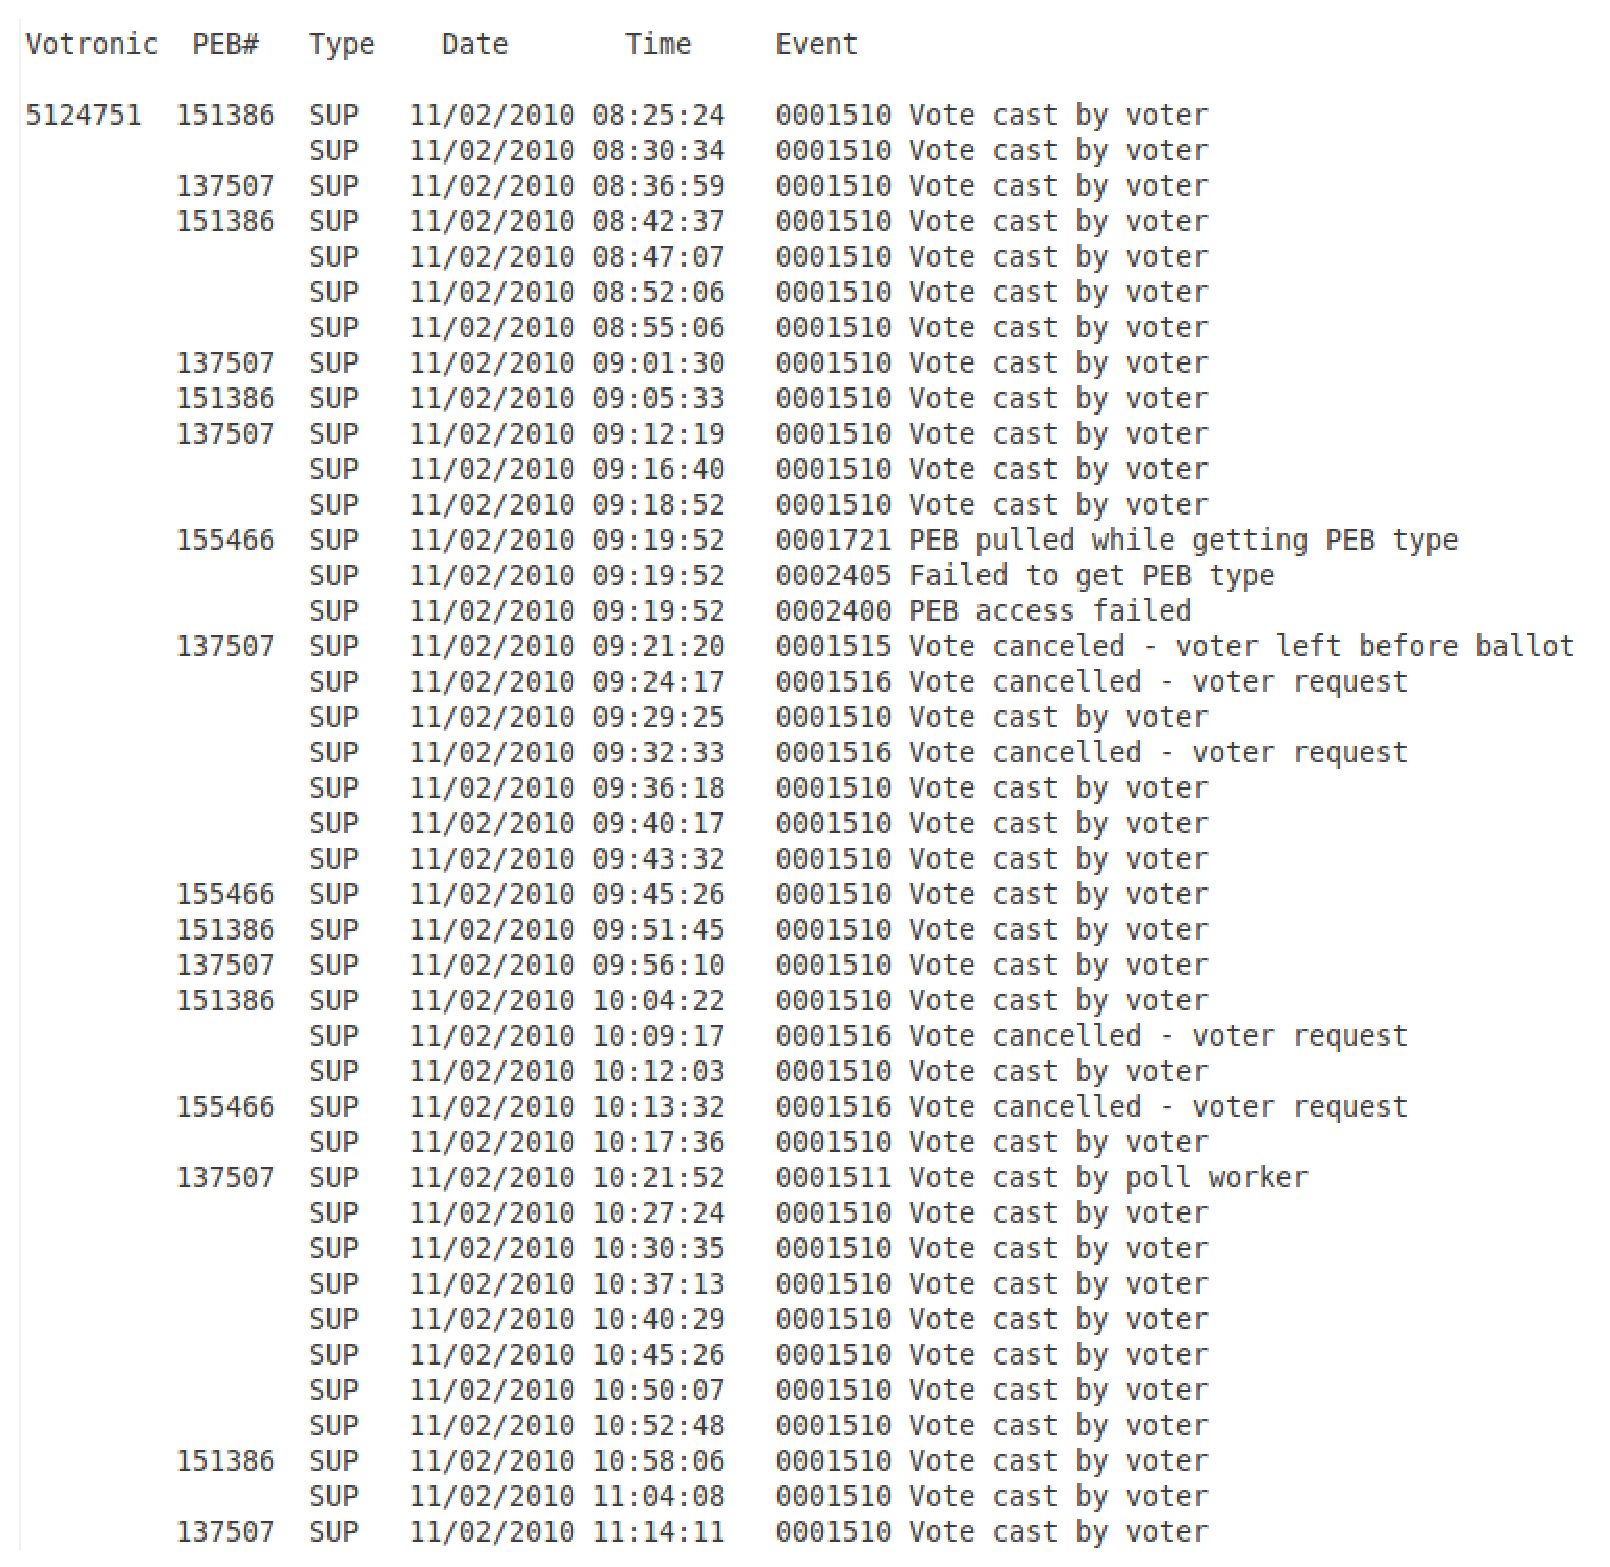
\includegraphics[width=0.8\textwidth]{eventLog}
%~\ref{app:el}

\clearpage
\section{Ballot Image File}\label{app:bi}
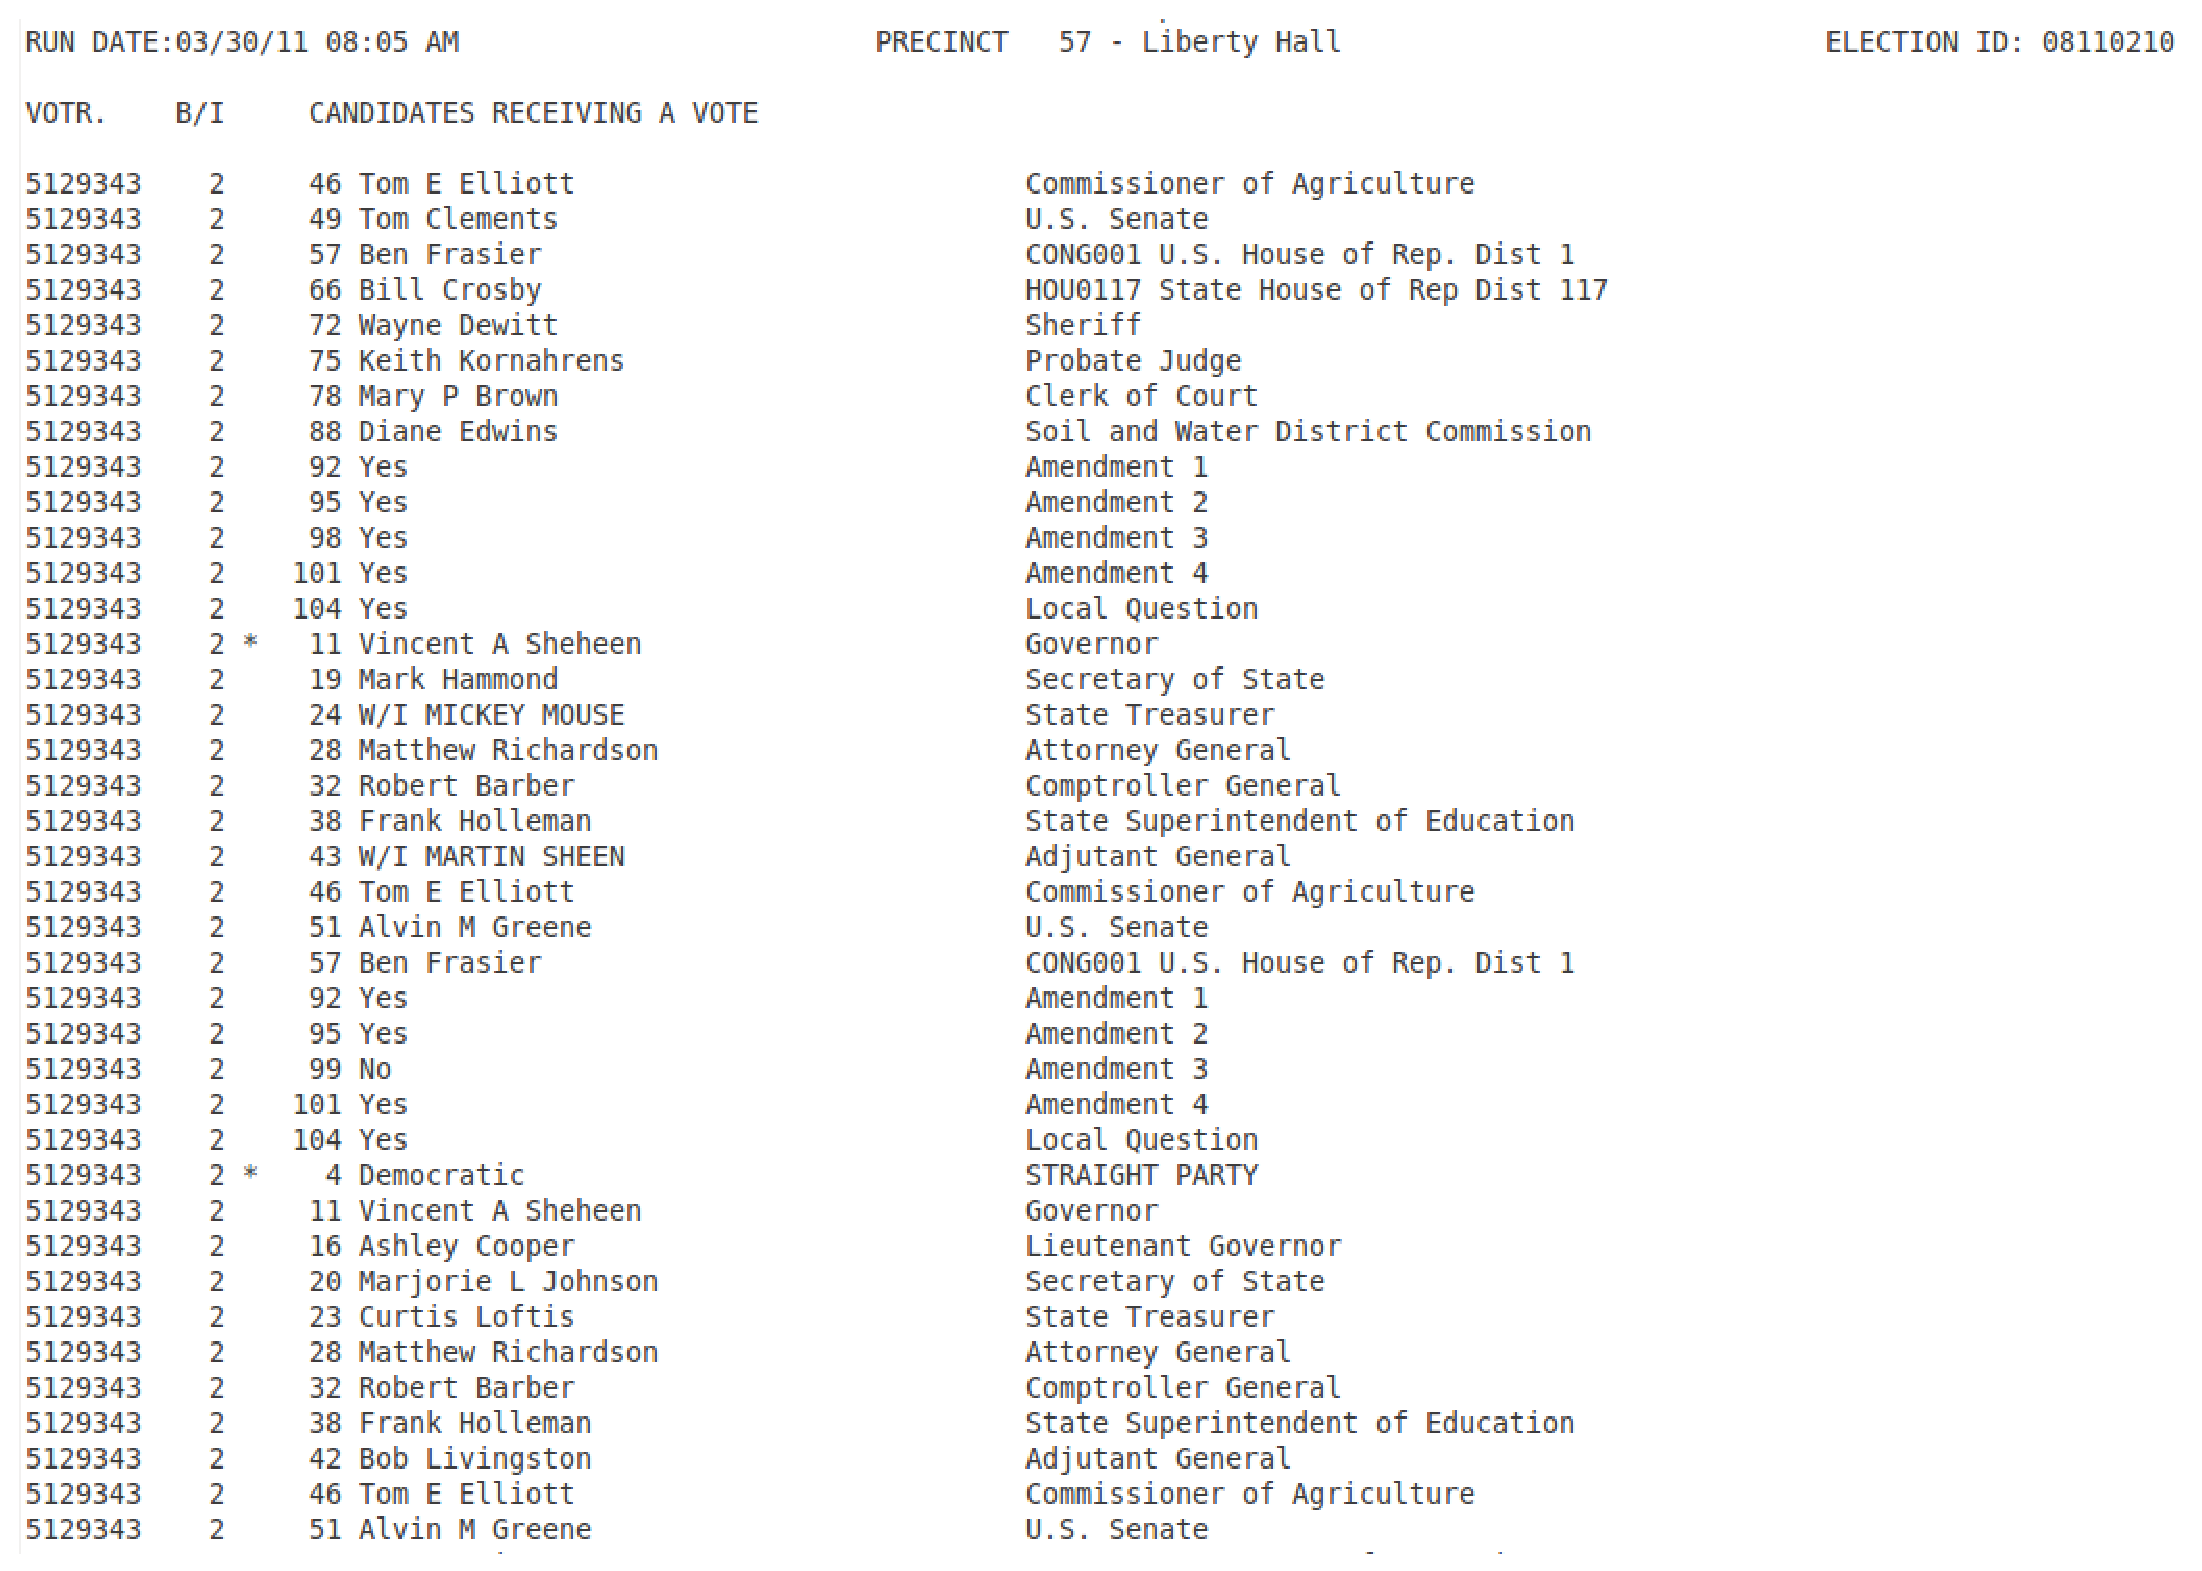
\includegraphics[width=0.9\textwidth]{ballot}
%This is app~\ref{app:bi}

\clearpage
\section{System Log File}\label{app:sl}
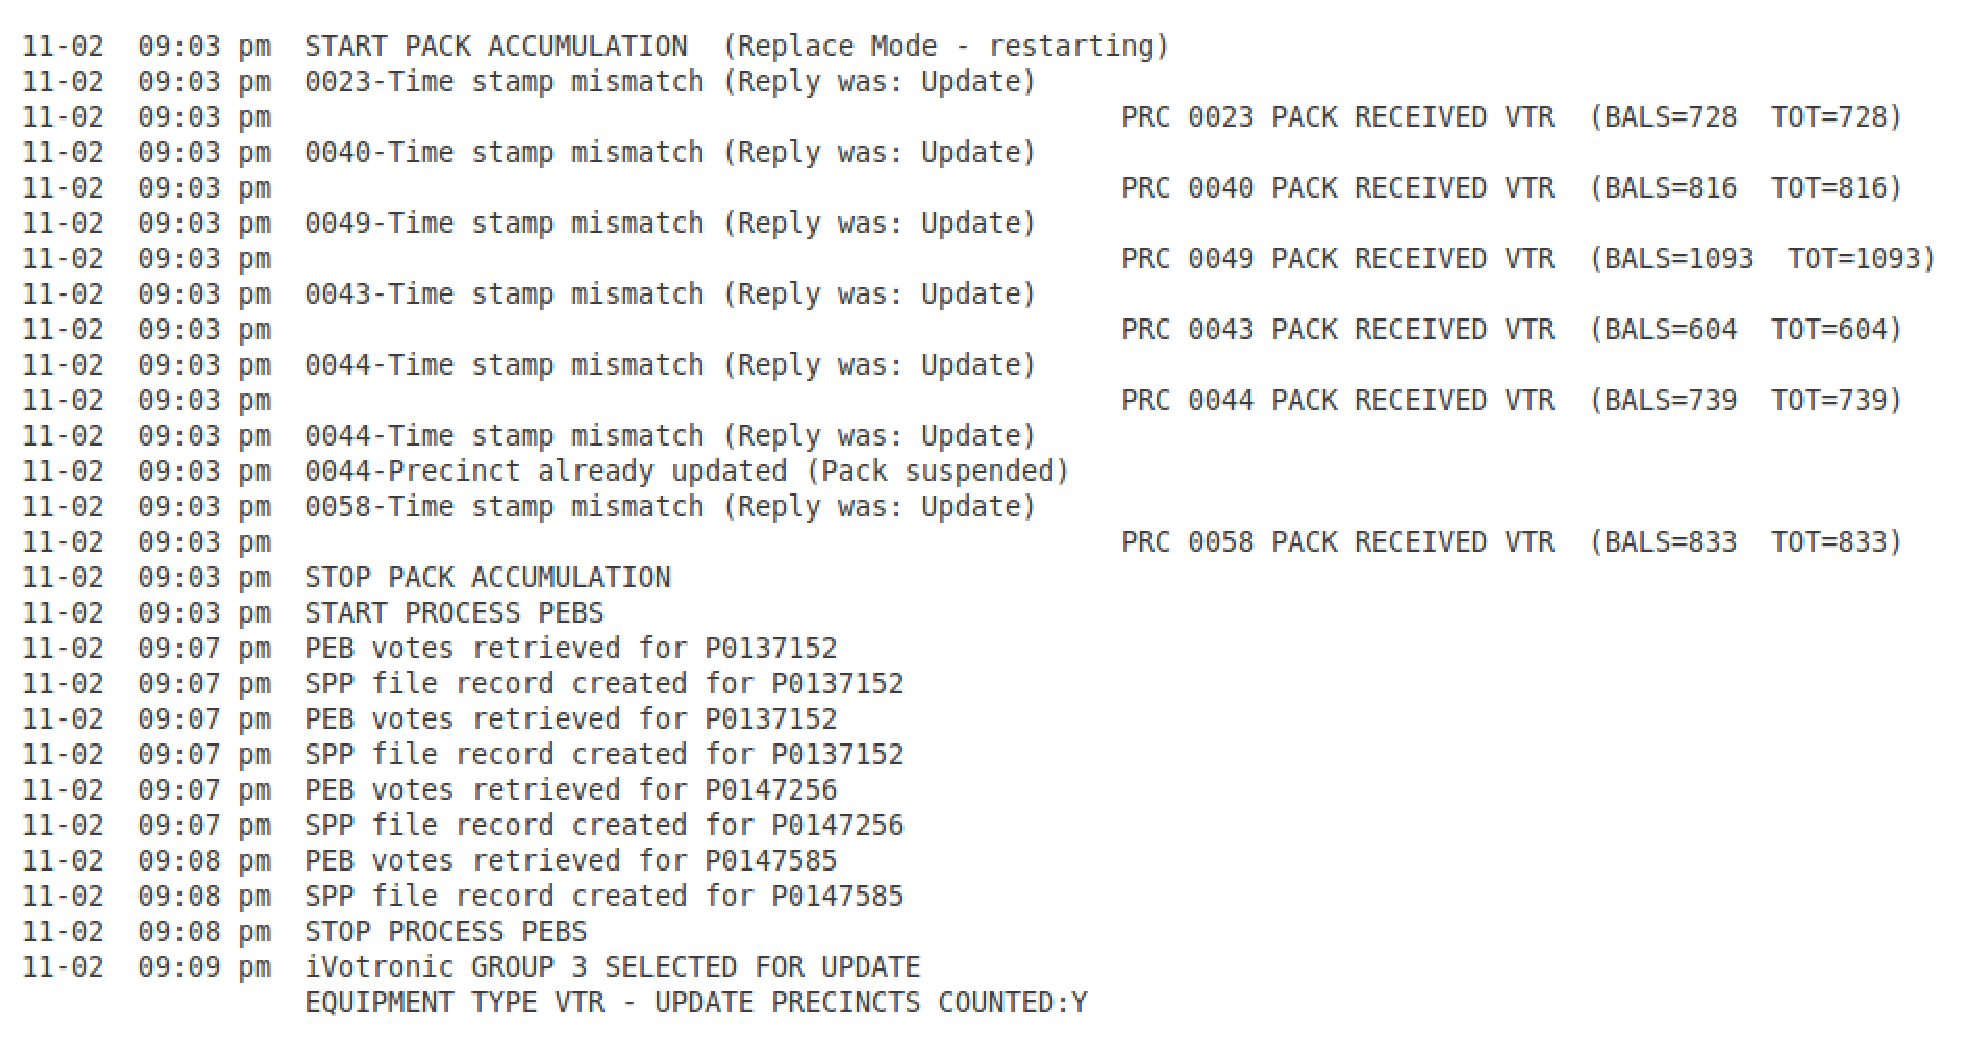
\includegraphics[width=0.9\textwidth]{system}
%This is app~\ref{app:sl}
\end{center}


\end{document}
